\graphicspath{ {./figures/} }
\section{Experiments \label{experiments}}
    \subsection{Environment}
        \begin{itemize}
            \item Python 3.8 was the language used for developing the machine learning models. 
            \item The libraries used to implement the models were Tensorflow 2.4, Keras, and Jupyter Notebook to help with the visualization.
            \item The models were trained on a Dell Poweredge R940XA Server that had 2 Intel Xeon Gold 5122 processors, 256GB of RAM, 2 NVIDIA Tesla V100 32G Passive GPU, and a 2TB HDD.
            \item The server ran a Docker container with the Ubuntu 18.04.4 LTS OS.
        \end{itemize}
    \subsection{Datasets}
        \begin{itemize}
            \item The data used for training the models were obtained from the PubChem database (REF).
            \item Using the PubChem REST API we were able to generate a dataset of $\sim$1.33 million entries.
            \item These entries were randomly chosen from the database.
            \item Each entry contained the following information: CID (the unique identifier used by PubChem), molecular formula, canonical SMILES, isometric SMILES, molecular weight, XLogP, exact mass, TPSA, complexity.
            \item For training all the models the canonical SMILES were used as input and for the third model fragments were used as well.
            \item The canonical SMILES was preferred since it gave us enough information about the molecular structure and helped ensure that each compound had a unique SMILES string.
            \item Most of the SMILES strings had a length of less than 200, with the average length being around 56.
            \item Since the SMILES consisted of the symbols of the elements and special characters with no white-space, instead of sentences, we considered more effective to tokenize the strings at character level before being given as input to the model. 
            \item It was then converted into a vector and given padding to ensure they all had the same length.
            \item The fragments used as input were generated using the RECAP technique.
            \item Fragments are similar to SMILES string, but instead represent the compound as a set of smaller SMILES strings.
            \item To generate the fragments we used the RDKit \cite{rdkit} Python library.
            \item When generated they were stored as a string where each fragment was separated by a white-space.
            \item Since not all of the compounds generated a set of fragments, then when not available the SMILES string was used instead. Acting as a single fragment.
            \item Most of the fragments generated also had a length of less than 200, with an average length of 144 characters. 
            \item These fragment strings were processed the same way as the SMILES strings.
            \item They were tokenized at a character level, vectorized, and given a padding.
            \item The molecular weight and XLogP of the compounds were also important as they were necessary to establish how good predictions of the models were.
            \item The molecular weights from the dataset ranged from $\sim$1 to $\sim$10,000 g/mol, with the average being at $\sim$439.44 g/mol.
            \item The XLogP from the dataset ranged from $\sim$-70 to $\sim$161, with the average being at $\sim$4.58.
            \item The dataset was split into 3 subsets: training, validation, and test sets. 
            \item The training set consisted of 600,000 elements of the data and was used for training the model.
            \item The validation set consisted of 200,000 elements of the data and was used while training to help fit the hyperparameters of the model.
            \item Finally, the test set consisted of 200,000 elements of the data was used to evaluated the model after training.
            \item The data that was not used was saved for any further testing we might want to do on the model.
        \end{itemize}
    % Not sure what to call this section, maybe Methodology?
    \subsection{Training the Models}
    \begin{itemize}
        \item The first model implemented was the one for predicting the molecular weight of a compound.
        \item Initially the padding used for the input data was 300, but was later changed to 1000 since this better accommodated for some of the much longer SMILES strings present in the dataset.
        \item Also the units for the fully connected layers were both 300, before reaching the final dense layer. 
        \item The results of this model, shown in Figures \ref{fig:model2-mol-weight-loss} and \ref{fig:model2-mol-weight-predictions}, were promising as a result we proceeded to tune it.
        \item To tune the model we used the Python library Talos (REF), which permitted us to tune various hyperparameters.
        \item Some of the initial hyperparameters tuned were: learning rate, epochs, and batch size. \item Later more parameters were included like the amount of units for layers and the kernel size in the convolutional layers.
        \item The resulting model is the one described in section \ref{archi}, which gave us the results shown in Figures \ref{fig:model20-mol-weight-loss} and \ref{fig:model20-mol-weight-predictions}.
        \item It was noted that the different models trained tended to do good at a subsection of the dataset given, but had higher error with larger molecular weights.
        \item This was likely the result of the distribution of the data as very little of the data was larger than 2,000 g/mol.
        \item Due to this a few models were trained using only data within 0 and 2,000 g/mol, to see if we could get more precise results in this smaller range.
        \item The results of the best out of those models can be seen in Figures \ref{fig:model23-mol-weight-loss} and \ref{fig:model23-mol-weight-predictions}
        \item Using this model as a guide we proceeded to develop the next two model for predicting the XLogP value of chemical compounds.
        \item The second model followed the same architecture as the previous, but was tuned so it would be more suited for prediction XLogP, hence why their architecture are so similar.
        \item The results of this model can be seen in Figures \ref{fig:model7-xlogp-loss} and \ref{fig:model7-xlogp-predictions}.
        \item Finally, the last model was implemented also using the first one as a base, and gave us the results in Figures \ref{fig:frag2-xlogp-loss} and \ref{fig:frag2-xlogp-predictions}.
    \end{itemize}
    
    % Figures
    % Initial molecular weight model results
    \begin{figure}
        \centering
        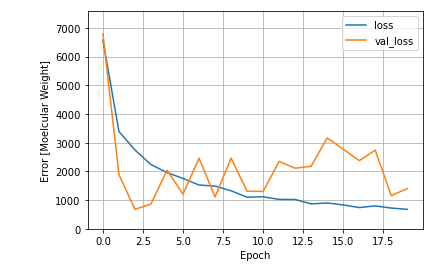
\includegraphics[width=0.5\textwidth]{loss_gragh_20_epoch.PNG}
        \caption{The loss graph of the first trained model for predicting molecular weight.}
        \label{fig:model2-mol-weight-loss}
    \end{figure}
    \begin{figure}
        \centering
        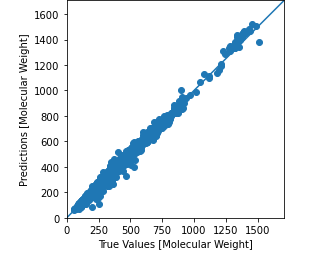
\includegraphics[width=0.5\textwidth]{model_2_prediction.PNG}
        \caption{Results of the first trained model for predicting molecular weight.}
        \label{fig:model2-mol-weight-predictions}
    \end{figure}
    
    % Best molecular weight model results
    \begin{figure}
        \centering
        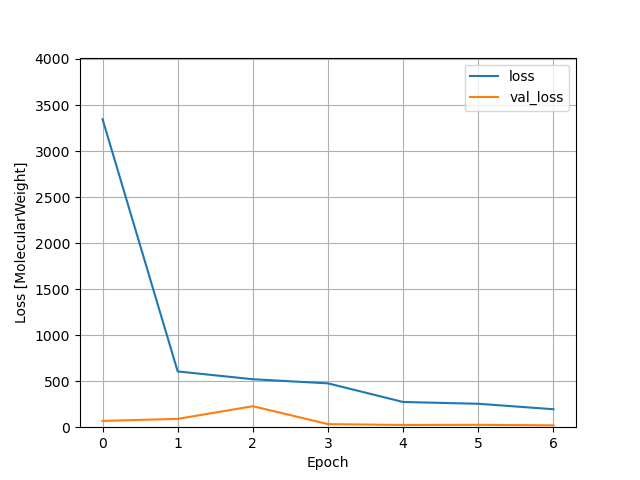
\includegraphics[width=0.5\textwidth]{model_20_7_epochs_loss_MolecularWeight.png}
        \caption{Loss graph of the latest tuned model for predicting molecular weight.}
        \label{fig:model20-mol-weight-loss}
    \end{figure}
    \begin{figure}
        \centering
        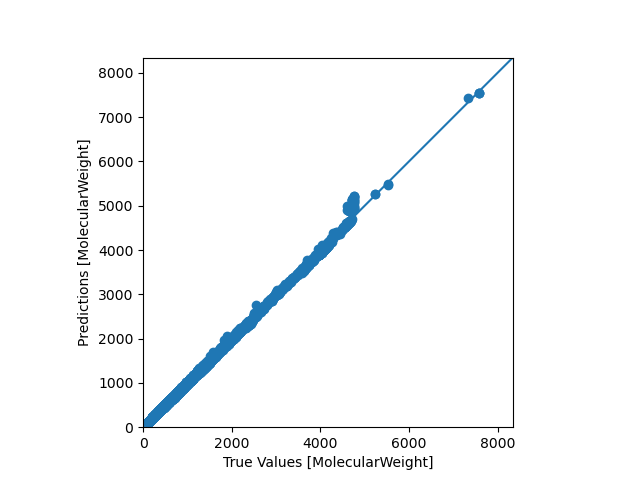
\includegraphics[width=0.5\textwidth]{model_20_7_epochs_predictions_MolecularWeight.png}
        \caption{Results latest tuned model for predicting molecular weight.}
        \label{fig:model20-mol-weight-predictions}
    \end{figure}
    
    % Best molecular weight < 2000 model results
    \begin{figure}
        \centering
        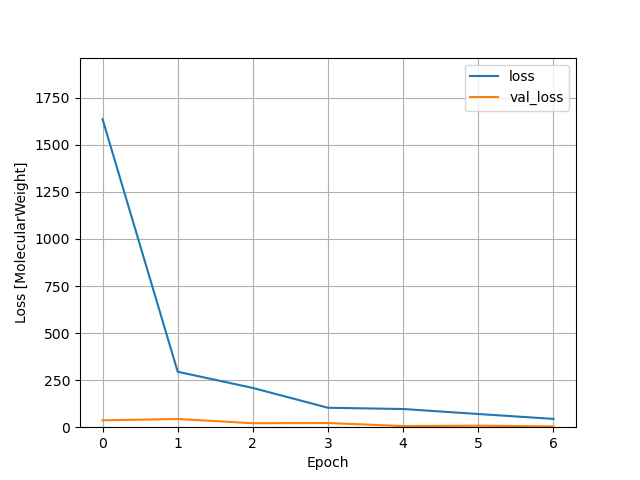
\includegraphics[width=0.5\textwidth]{model_23_7_epochs_loss_MolecularWeight.png}
        \caption{Loss graph of the latest tuned model for predicting molecular weight.}
        \label{fig:model23-mol-weight-loss}
    \end{figure}
    \begin{figure}
        \centering
        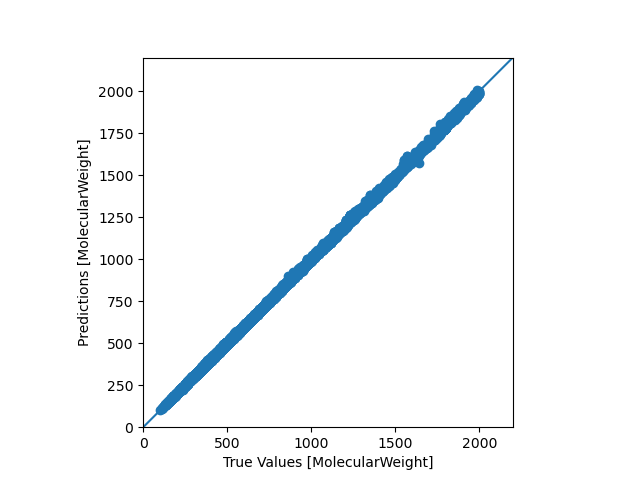
\includegraphics[width=0.5\textwidth]{model_23_7_epochs_predictions_MolecularWeight.png}
        \caption{Results latest tuned model for predicting molecular weight.}
        \label{fig:model23-mol-weight-predictions}
    \end{figure}
    
    % Best XLogP model results
    \begin{figure}
        \centering
        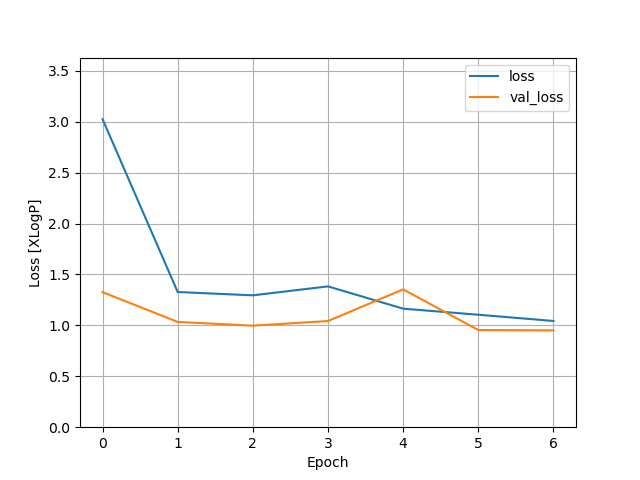
\includegraphics[width=0.5\textwidth]{model_7_7_epochs_loss_XLogP.png}
        \caption{Loss graph of the model trained for predicting XLogP.}
        \label{fig:model7-xlogp-loss}
    \end{figure}
    \begin{figure}
        \centering
        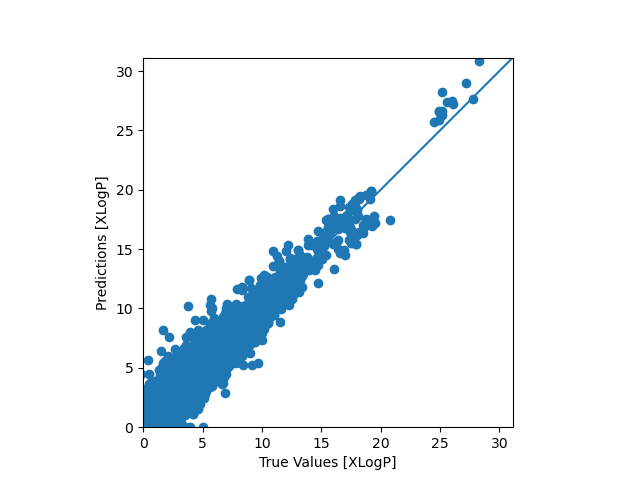
\includegraphics[width=0.5\textwidth]{model_7_7_epochs_predictions_XLogP.png}
        \caption{Results of the model trained for predicting XLogP.}
        \label{fig:model7-xlogp-predictions}
    \end{figure}
    
    % Fragment XLogP model results
    \begin{figure}
        \centering
        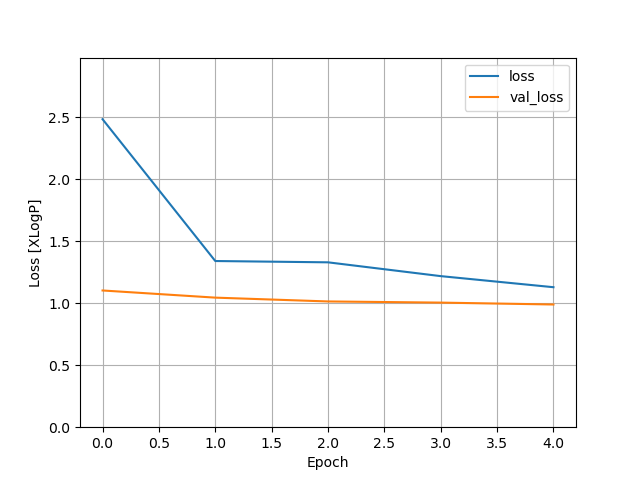
\includegraphics[width=0.5\textwidth]{figures/XLogP_model_2_5_epochs_loss.png}
        \caption{Loss graph of the model that used SMILES and fragments as input for predicting XLogP.}
        \label{fig:frag2-xlogp-loss}
    \end{figure}
    \begin{figure}
        \centering
        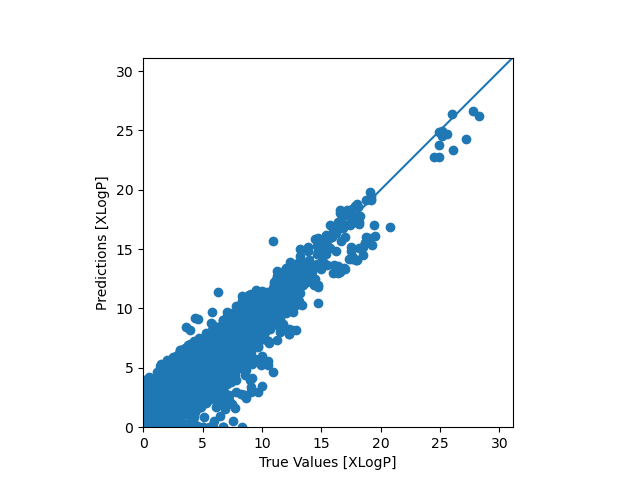
\includegraphics[width=0.5\textwidth]{figures/XLogP_model_2_5_epochs_predictions.png}
        \caption{Results of the model that used SMILES and fragments as input for predicting XLogP.}
        \label{fig:frag2-xlogp-predictions}
    \end{figure}
    
    \subsection{Results}
    \begin{itemize}
        \item 
    \end{itemize}
    % Figures
    \begin{figure}
        \centering
        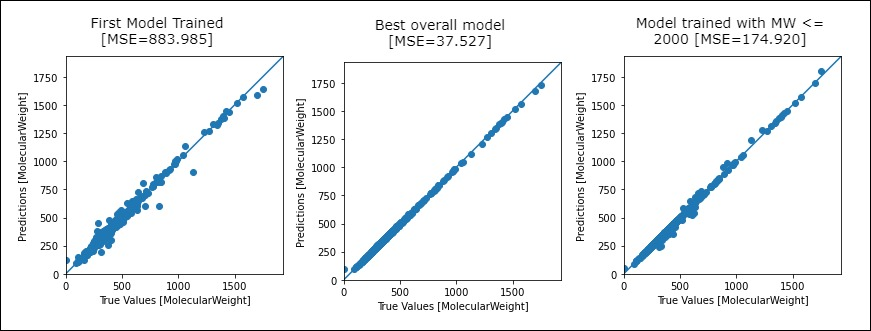
\includegraphics[width=0.5\textwidth]{figures/graphs-Mol-Wei_Comp1.jpg}
        \caption{Comparison of results of the three models that predict the molecular.}
        \label{fig:comparison_mol_weight}
    \end{figure}
    \begin{figure}
        \centering
        \includegraphics[width=0.5\textwidth]{}
        \caption{}
        \label{fig:model2-mol-weight-predictions}
    \end{figure}
    \begin{figure}
        \centering
        \includegraphics[width=0.5\textwidth]{}
        \caption{}
        \label{fig:model20-mol-weight-loss}
    \end{figure}
    \begin{figure}
        \centering
        \includegraphics[width=0.5\textwidth]{}
        \caption{}
        \label{fig:model20-mol-weight-predictions}
    \end{figure}